%
% Sección de algoritmos implementados,
% Presentación de TT1.
%
% Proyecto Lovelace.
%

\subsection{Implementaciones}

\begin{frame}{Algoritmos implementados}

  \begin{itemize}
    \item<1-> Reversibles:
      \begin{itemize}

        \item<2-> FFX (\textit{Fortmat-preserving Feistel-basen Encryption}).
          Publicado por Mihir Bellare, Phillip Rogaway y Terence Spies en
          \cite{ffx_1}.

          \note<2>
          {
            Es una propuesta de estándar para el NIST. Los autores son los
            principales precursores de los cifrados que preservan el
            formato.

            El método está basado en redes Feistel y una función de ronda
            que ocupa CBC-MAC-AES.
          }

        \item<3-> BPS. Publicado por Eric Brier, Thomas Peyrin y Jacques
          Stern en \cite{bps}.

          \note<3>
          {
            También es propuesta de estándar para el NIST. Representa la
            principal competencia de FFX.

            Al igual que FFX, ocupa redes Feistel de forma interna; se
            diferencian en algunos detalles de instanciación y en que
            BPS está diseñado para cadenas de longitud arbitraria.
          }

      \end{itemize}
    \item<4-> Irreversibles:
      \begin{itemize}

        \item<5-> TKR. Publicado por Sandra Díaz-Santiago, Lil María
          Rodríguez-Henríquez y Debrup Chakraborty en \cite{doc_sandra}.

          \note<5>
          {
            El documento es el primer análisis formal sobre la generación de
            tokens. TKR es el primer método propuesto (cuya seguridad está
            formalente probada) que no es un cifrado que preserva el formato.
          }

        \item<6-> AHR (Algoritmo Híbrido Reversible). Longo, Aragona y Sala
          en \cite{aragona}.

        \item<7-> DRBG (\textit{Deterministic Random Bit Generator}). Adaptación
          a aprtir de estándar del NIST (\textit{National Institute of Standards
          and Technology}) \cite{nist_aleatorios}.

          \note<7>
          {
            En la gran mayoría de los casos se buscó no hacer implementaciones
            propias de primitivas criptográficas, sin embargo, en el caso del
            generador, se hizo un excepción, para darle un poco más de contenido
            al trabajo. Esto último dado que hacer un generador implica también
            validarlo con pruebas de aleatoriedad del NIST.
          }

      \end{itemize}
  \end{itemize}
\end{frame}

\begin{frame}{Diseño de programa}{Componentes}

  \begin{figure}[H]
    \begin{center}
      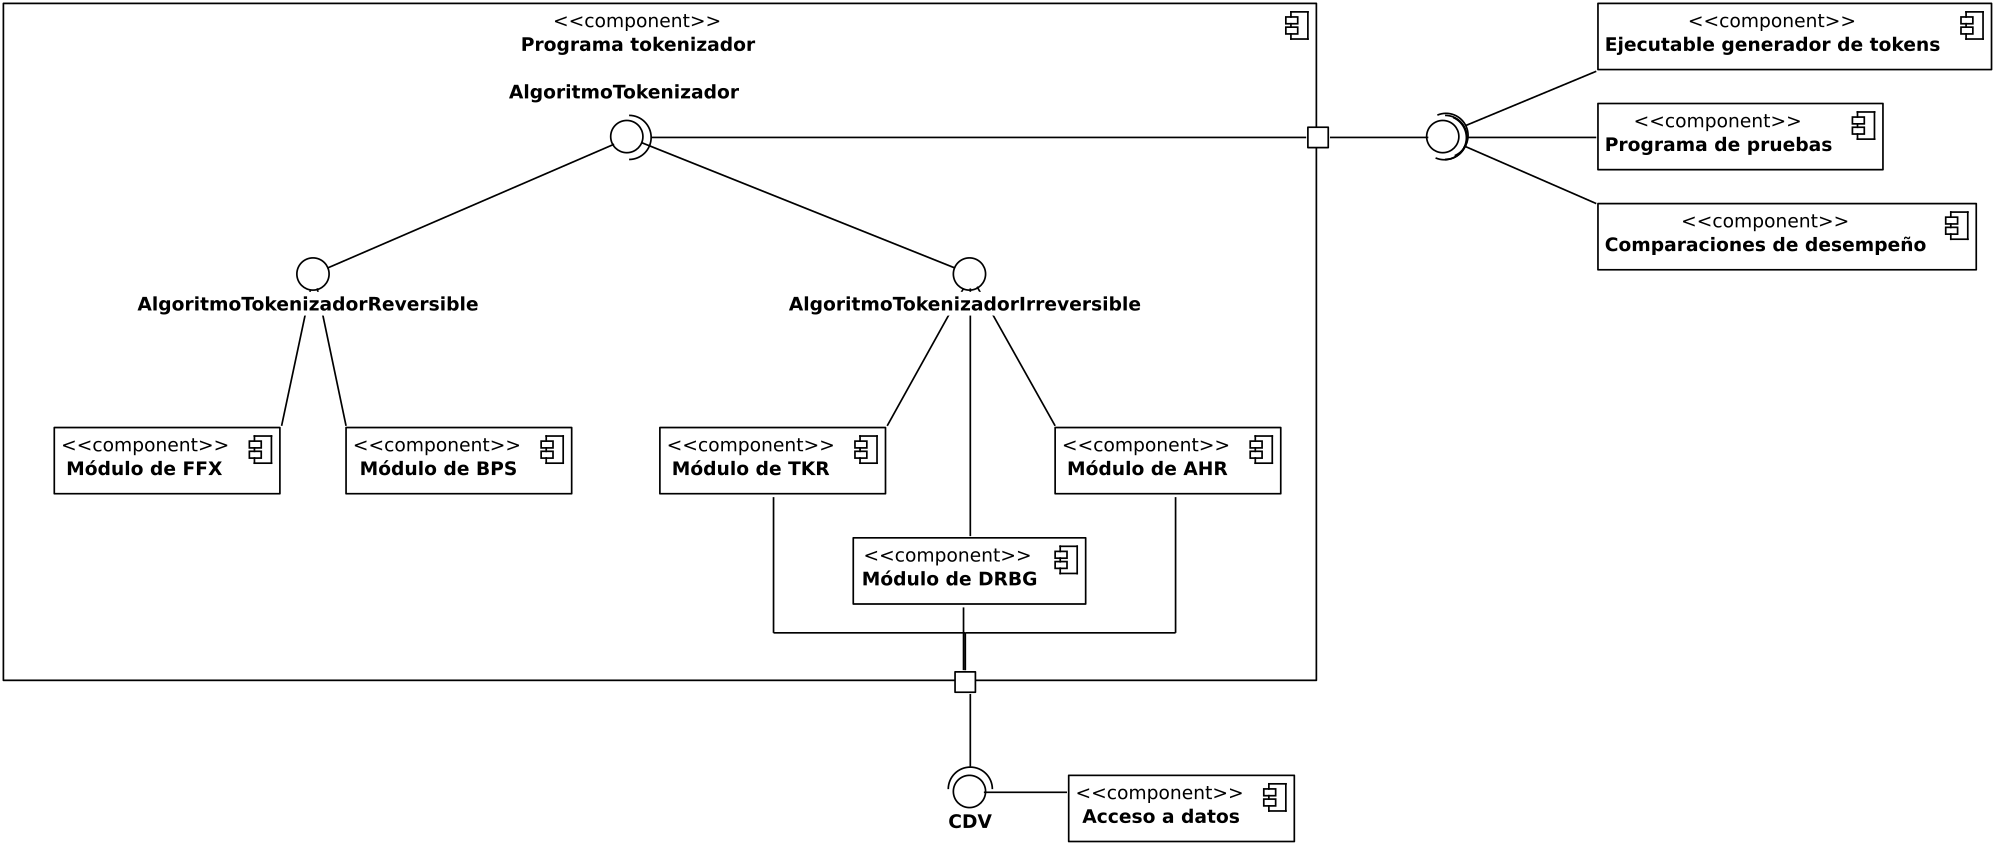
\includegraphics[width=1.0\linewidth]
        {../../../diagramas_comunes/disenio/componentes.png}
      \caption{Diagrama de componentes del programa.}
    \end{center}
  \end{figure}

  \note
  {
    Se muestra la estructura interna del componenete del programa
    tokenizador. Aunque adentro de este hay varios módulos, a las entidades
    externas solo les interesa comunicarse a través de la interfaz. El acceso
    a datos se maneja también a través de una interfaz externa al componente;
    los método irreversibles deben tener acceso a esta.
  }

\end{frame}
